%
% loesung.tex -- Beispiel-File für die Beschreibung der Loesung
%
% (c) 2020 Prof Dr Andreas Müller, Hochschule Rapperswil
%
\section{Lösung
\label{vanderpol:section:loesung}}
\rhead{Lösung}
Der vorhergehende Abschnitt beschreibt die Antwort des Systems auf die Änderung der Anfangsbedingungen. Stattdessen soll nun analysiert werden, wie die Lösung der Gleichung \ref{vanderpol:equations:vdp} auch durch die Länge des Integrationsschrittes beeinflusst werden kann. Zuvor sind jedoch die verschiedenen Implementierungen der wichtigsten verwendeten Codes aufgelistet.
\subsection{Implementierungen 
\label{vanderpol:subsection:implementierungen }}
\lstinputlisting[style=Python,caption={Implementierung des Runge-Kutta-Algorithmus in Python}, captionpos={b}, label={vanderpol:codes:RK_4}]{papers/vanderpol/codes/RK_4.py}
Der Codeabschnitt \ref{vanderpol:codes:RK_4} stellt die Python-Implementierung des Runge-Kutta-Algorithmus vierter Ordnung vor. Die Koeffizienten werden gemäss der nachstehenden analytischen Definition berechnet:

\begin{align*}
k_1 &= h \cdot f(t_n, y_n) \\
k_2 &= h \cdot f\left(t_n + \frac{h}{2}, y_n + \frac{h}{2} k_1\right) \\
k_3 &= h \cdot f\left(t_n + \frac{h}{2}, y_n + \frac{h}{2} k_2\right) \\
k_4 &= h \cdot f(t_n + h, y_n + h k_3) \\
\end{align*}
und dann wird der gewichtete Durchschnitt wie nachstehend ermittelt:

\begin{equation}
y_{n+1} = y_n + \frac{1}{6}(k_1 + 2k_2 + 2k_3 + k_4) +O(h^5)
\end{equation}
Der Code des Euler Algorithmus wurde nicht berichtet, denn es handelt sich um eine vereinfachte Version des Codes im Abschnitt \ref{vanderpol:codes:RK_4}, in dem nur der Koeffizient $k_1$ berechnet werden muss. Da dies ein einziger Wert ist, ist es nicht notwendig, einen Mittelwert zu bilden. Die Berechnung wird dann reduziert auf:

\begin{align*}
k_1 &= h \cdot f(t_n, y_n) \\
y_{n+1} &= y_n + k_1 +O(h^2)
\end{align*}

\break
\lstinputlisting[style=Python,caption={Implementierung der van der pol-Gleichung in Python}, captionpos={b}, label={vanderpol:codes:VDP_funk}]{papers/vanderpol/codes/VDP_funk.py}
Der Abschnitt \ref{vanderpol:codes:VDP_funk} zeigt stattdessen die Implementierung der Differentialgleichung \ref{vanderpol:equations:inhomogene_2}.  Die entwickelte Idee lautet wie folgt: In In beiden Fällen stellt die Variable $z_n$ einen Vektor dar, der die beiden Werte der Funktionen $x_n$ und $\dot{x}_n$ enthält. Letzteres ist somit dem aktuellen Zustand $n$. Beide Funktionen erhalten auch einen zweiten Eingabeparameter $t_n$, der dem aktuellen Zeitpunkt entspricht. Der Code in \ref{vanderpol:codes:VDP_funk} kümmert sich um die Definition der Differentialgleichung, die dann in der in \ref{vanderpol:codes:RK_4} eingeführten Funktion verwendet wird, um den Kutta-Runge-Algorithmus auszuführen und $x_{n+1}$ und $\dot{x}_{n+1}$ als Ausgabe zu erhalten.\\
Zusammengefasst werden die beiden Funktionen als Eingabe gegeben: ein bestimmter Zeitwert $t_n$, der aktuelle Wert der Funktion $x_{n}$ und ihre Ableitung $\dot{x}_{n}$. Es wird eine Ausgabe zurückgegeben, die dem nächsten Wert der Funktion $x_{n+1}$ und ihrer Ableitung $\dot{x}_{n+1}$ entspricht. Es wird in dieser Form dargestellt:

\begin{equation}
\begin{pmatrix}x_{n+1} \\ \dot{x}_{n+1} \end{pmatrix} = \begin{pmatrix}x_{n} \\ \dot{x}_{n} \end{pmatrix} + \frac{1}{6}(\vec{k_1} + 2\vec{k_2} + 2\vec{k_3} + \vec{k_4})
\label{vanderpol:equations:solve_alg}
\end{equation}
Die Konstanten von $k_1$ bis $k_4$ sind Vektoren, die die Koeffizienten für beide von uns benötigten Lösungen enthalten, nämlich $x_{n+1}$ und $\dot{x}_{n+1}$.
Diesen werden dann gleichzeitig berechnet. Dieser Algorithmus ist eine Implementierung der in \ref{vanderpol:equations:homogene_1} vorgestellten Substitution.
\lstinputlisting[style=Python,caption={Python-Algorithmus zur Berechnung der Lösung}, captionpos={b}, label={vanderpol:codes:solve}]{papers/vanderpol/codes/solve.py}
Die Implementierung des in der Gleichung \ref{vanderpol:equations:solve_alg} beschriebenen Verfahrens wird im Abschnitt des Codes \ref{vanderpol:codes:solve} gezeigt.
Um eine vollständige Lösung für einen beliebigen Bereich $[a, b]$ zu erhalten, muss man die darin enthaltenen Zeitwerte berechnen. Dieses Interval muss also diskretisiert werden, indem es in $n$ gleiche Teile aufgeteilt wird. Daraus ergibt sich eine Menge von Zeitwerten, die von $t_0$ bis $t_n$ läuft.
Dies ist genau das, was im Abschnitt code \ref{vanderpol:codes:solve} ausgeführt wird. Zu Beginn werden das Zeitintervall und die Anfangsbedingungen angegeben, ab denen die Iteration dann beginnt, was in diesem Fall zu einer Lösung von $t=0$ bis $t_n=950,0$ führt.

\subsection{Ergebnisse
\label{vanderpol:section:ergebnisse}}
Nachstehend sind die Ergebnisse der beiden oben beschriebenen Algorithmen aufgeführt. Die ausgewählten Anfangsbedingungen sind wie folgt:

\begin{itemize}
\item
$\dot{x_1}(0) = \dot{x_1}(0) = 5$
\item
$x_1(0) = x_2(0) = 0$
\end{itemize}
In diesem Fall wurden im Gegensatz zu den in Abb.\ref{vanderpol:figures:init_cond_VDP} gezeigten Daten zwei verschiedene Integrationsschritte gewählt. Die Ergebnisse sind jedoch fast die gleichen. Im Falle der Runge-Kutta Lösung wird deutlich, dass der Divergenzpunkt aufgrund der Änderung der Integrationsschritt noch vor dem liegt, der sich durch die Veränderung der Anfangsbedingungen ergibt. Auch in diesem Fall verursachte eine Differenz in der Grössenordnung von $10^{-3}$ eine starke Abweichung. Der Runge-Kutta-Algorithmus hat einen Rundungsfehler in der Grössenordnung von $O(h^5)$, während Euler $O(h^2)$ hat. Dies wirkt sich auf die Zeit $t_0$ aus, wenn Chaos eintritt. Im ersten Fall haben wir $t_0 \cong 770,5$ wie in Abb. \ref{vanderpol:figures:RK_schritt_e-3} gezeigt, während im zweiten Fall $t_0 \cong 59,7$ wie in Abb. \ref{vanderpol:figures:EULER_schritt} gezeigt.  

\begin{figure}
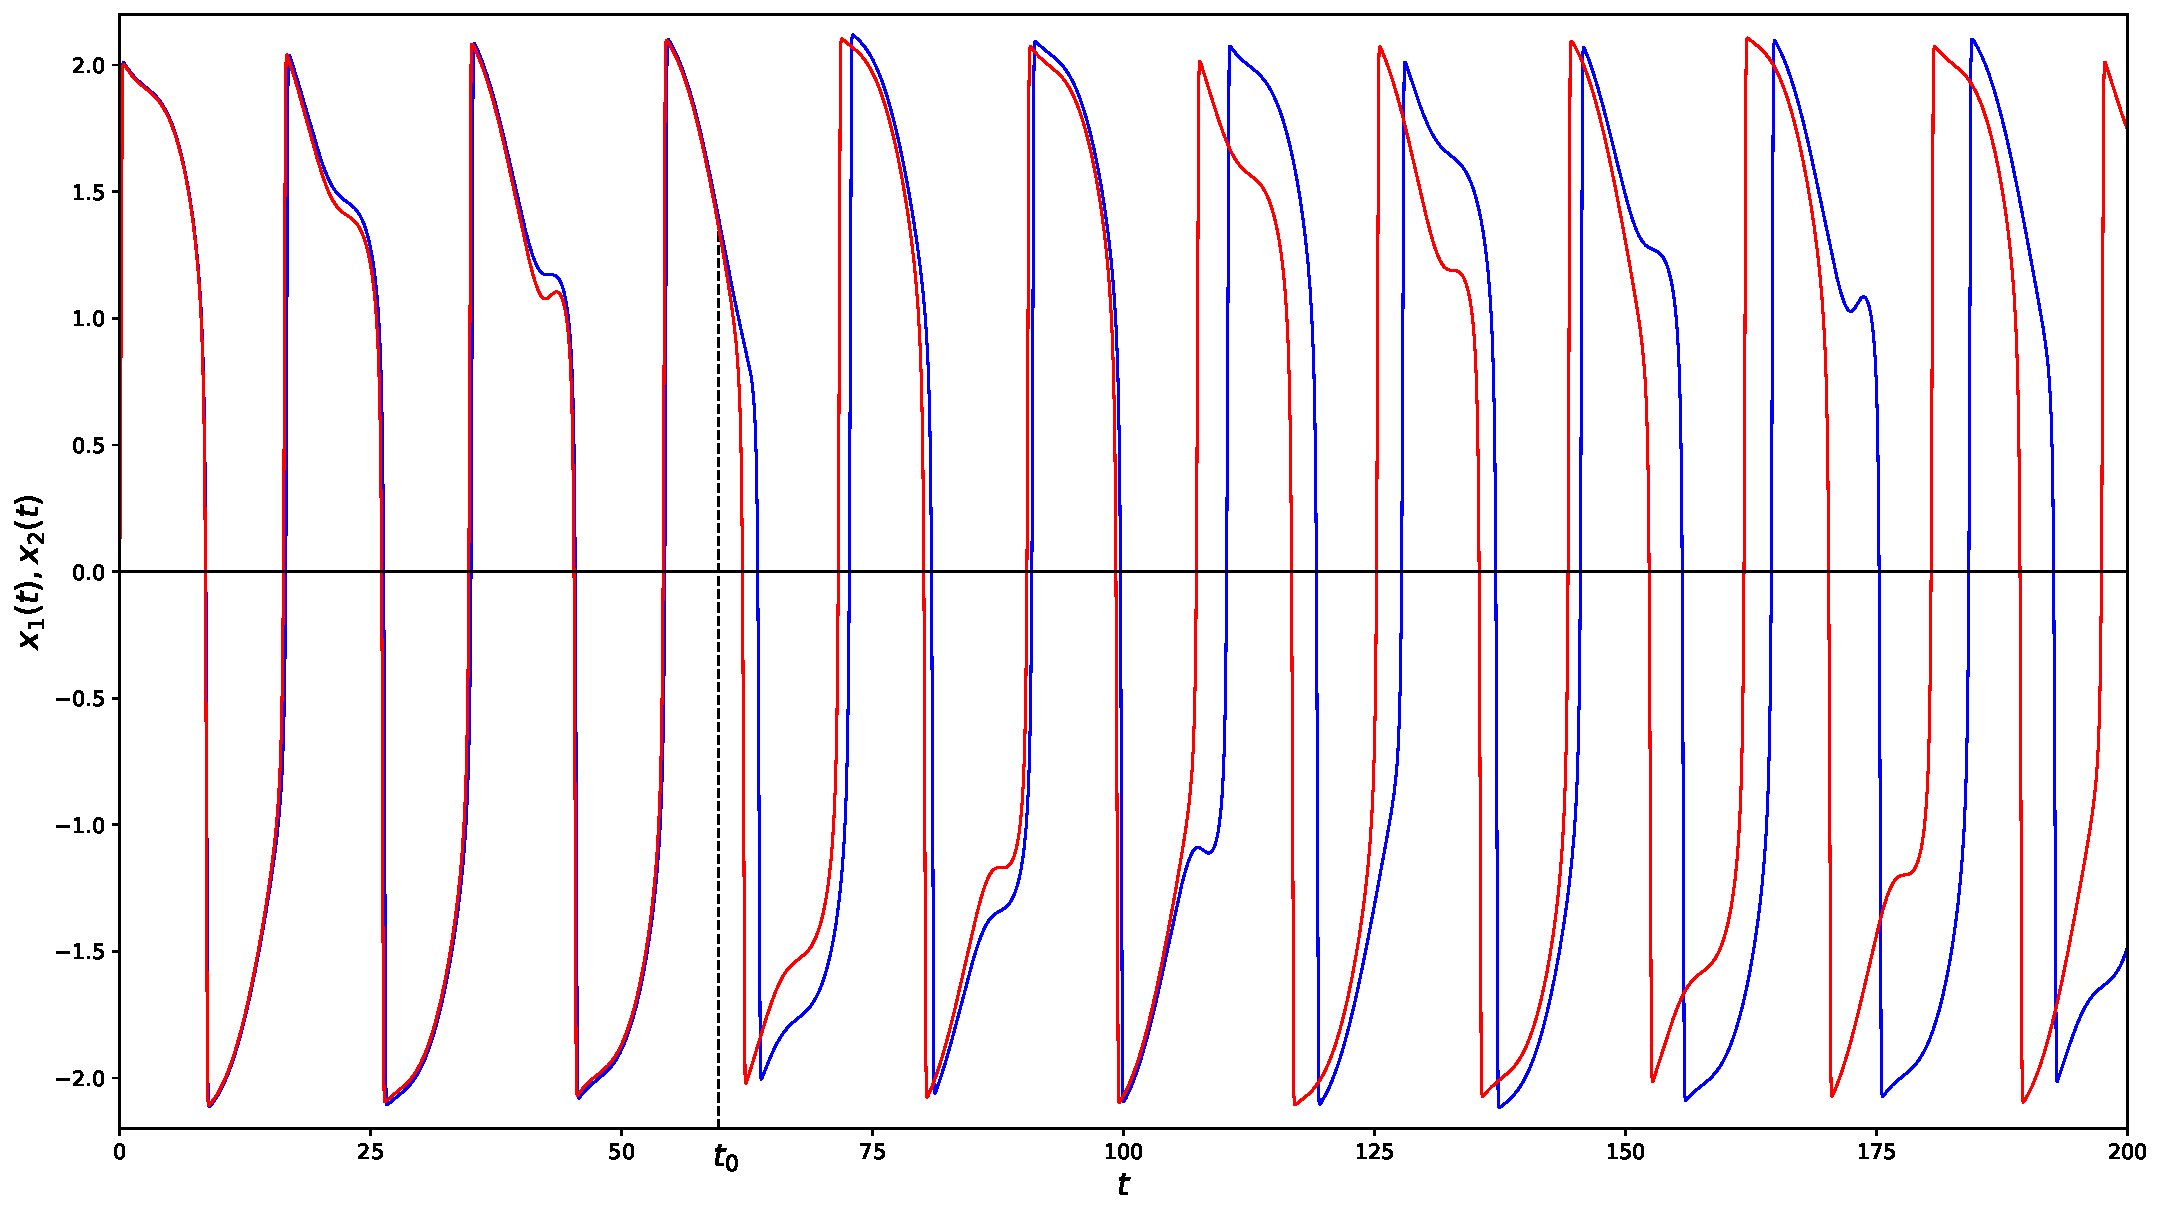
\includegraphics[width=\textwidth]{papers/vanderpol/figures/EULER_schritt_delta_e-3.pdf}
\caption{Verlauf der beiden mit der {\em Euler-Methode} berechneten Lösungen $x_1$ und $x_2$ im Zeitbereich und Angabe des Divergenzpunktes $t_0$. Integrationsschritte: $h_1 = 0.01, \quad h_2 = 0.009$\label{vanderpol:figures:EULER_schritt}}
\end{figure}

\begin{figure}
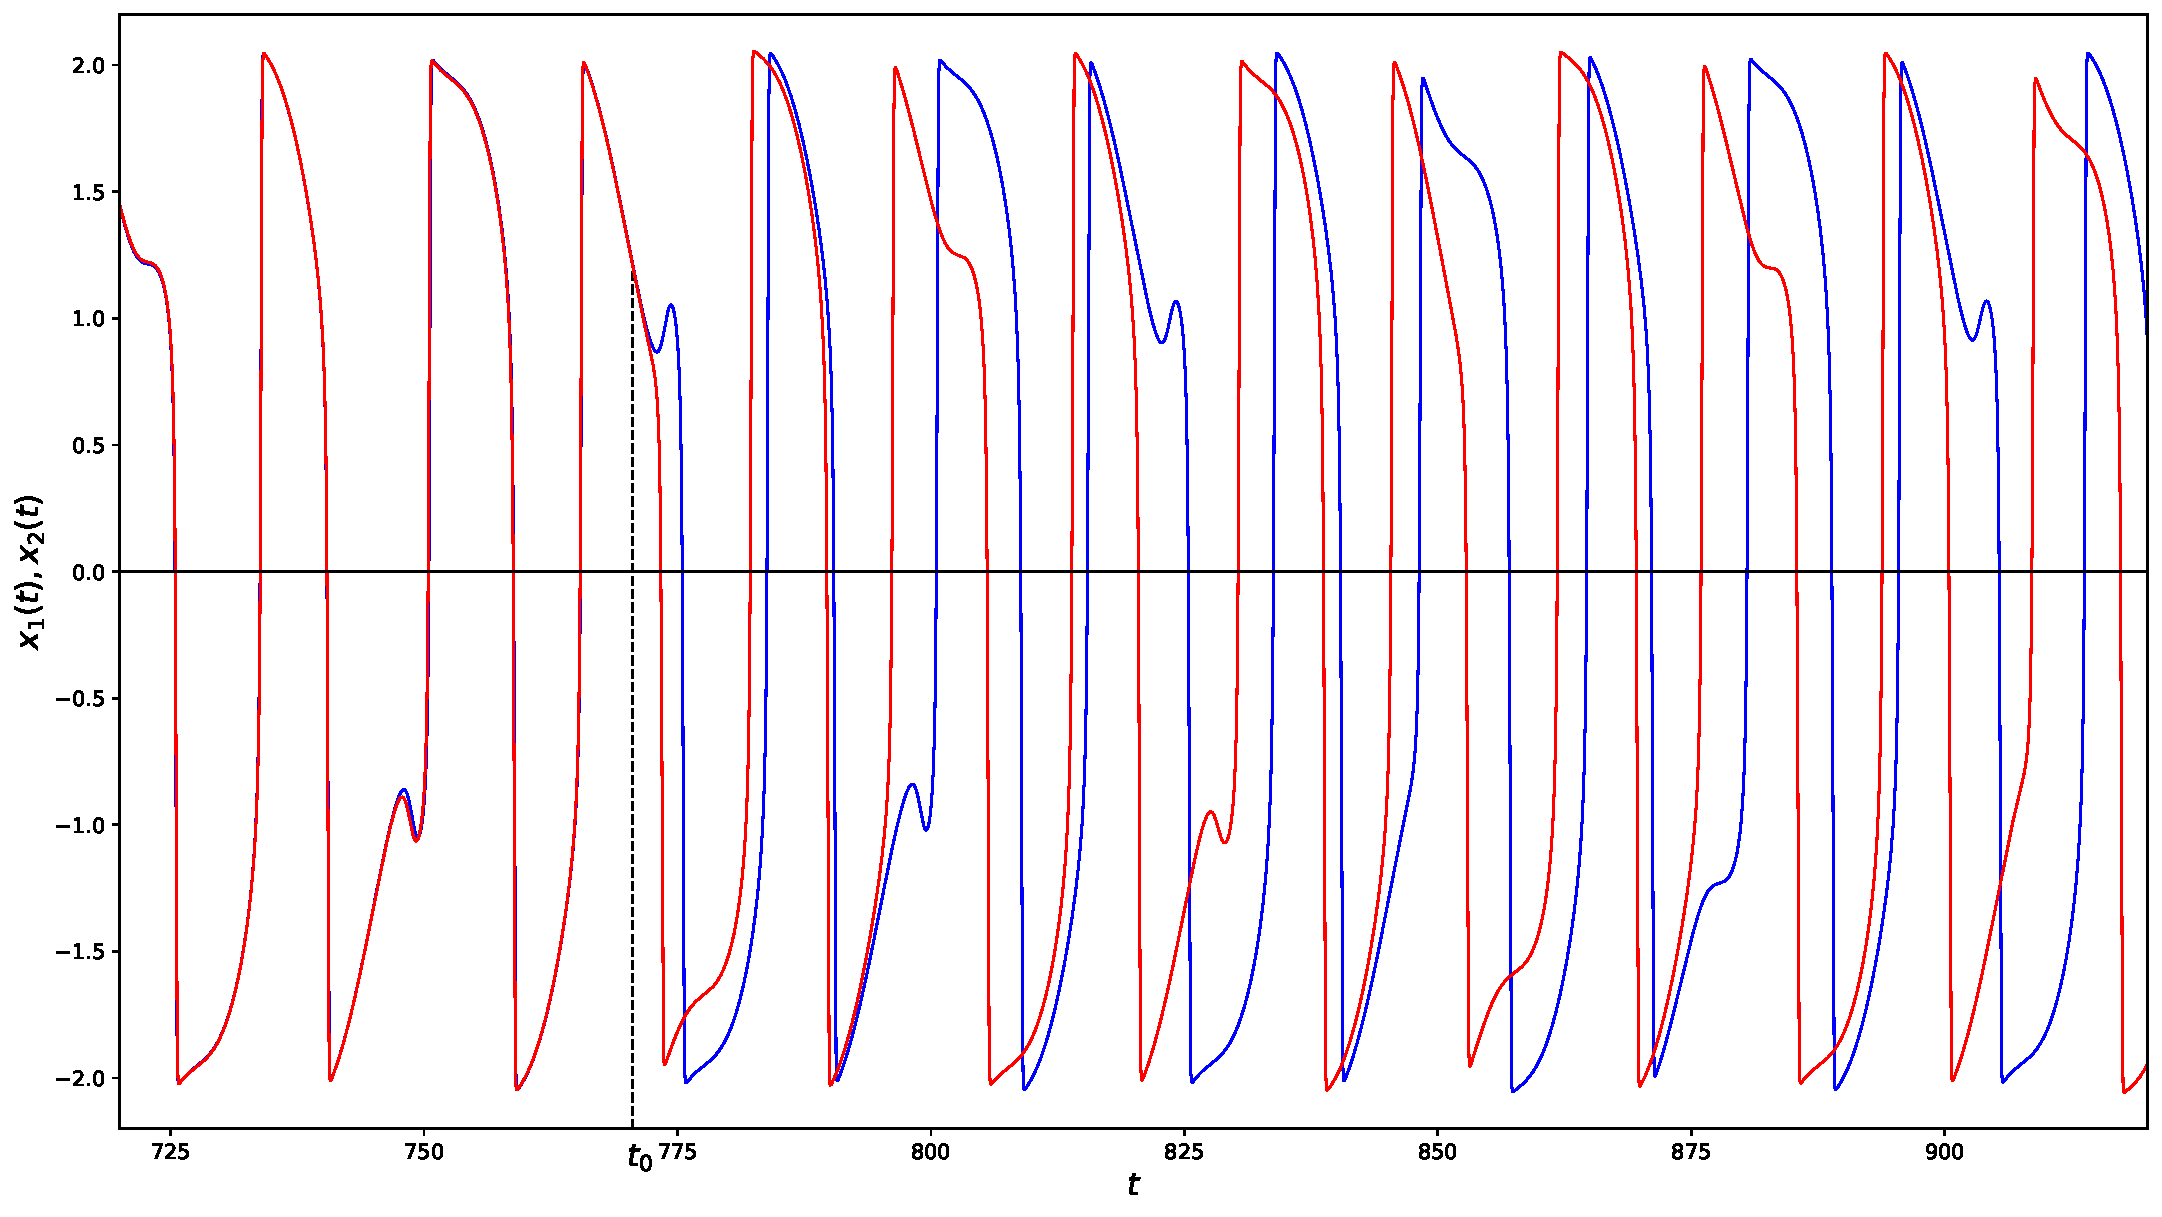
\includegraphics[width=\textwidth]{papers/vanderpol/figures/RK_schritt_delta_e-3.pdf}
\caption{Verlauf der beiden mit der {\em Runge-Kutta-Methode vierter Ordnung} berechneten Lösungen $x_1$ und $x_2$ im Zeitbereich und Angabe des Divergenzpunktes $t_0$. Integrationsschritte: $h_1 = 0.01, \quad h_2 = 0.009$\label{vanderpol:figures:RK_schritt_e-3}}
\end{figure}
In den folgenden Plots wird gezeigt, wie die Abnahme des Integrationsschrittes $h$ immer zu einem Divergenzpunkt $t_0$ führt, an dem das System chaotisch wird. Im Fall von Abb. \ref{vanderpol:figures:RK_schritt_2e-3} ist der Schritt $h_1=0.007$ und $h_2=0.009$ . In Abb. \ref{vanderpol:figures:RK_schritt_2e-3_2} wird die Schrittlänge auf $h_1=0.005$ und $h_2=0.007$ verringert.

\begin{figure}
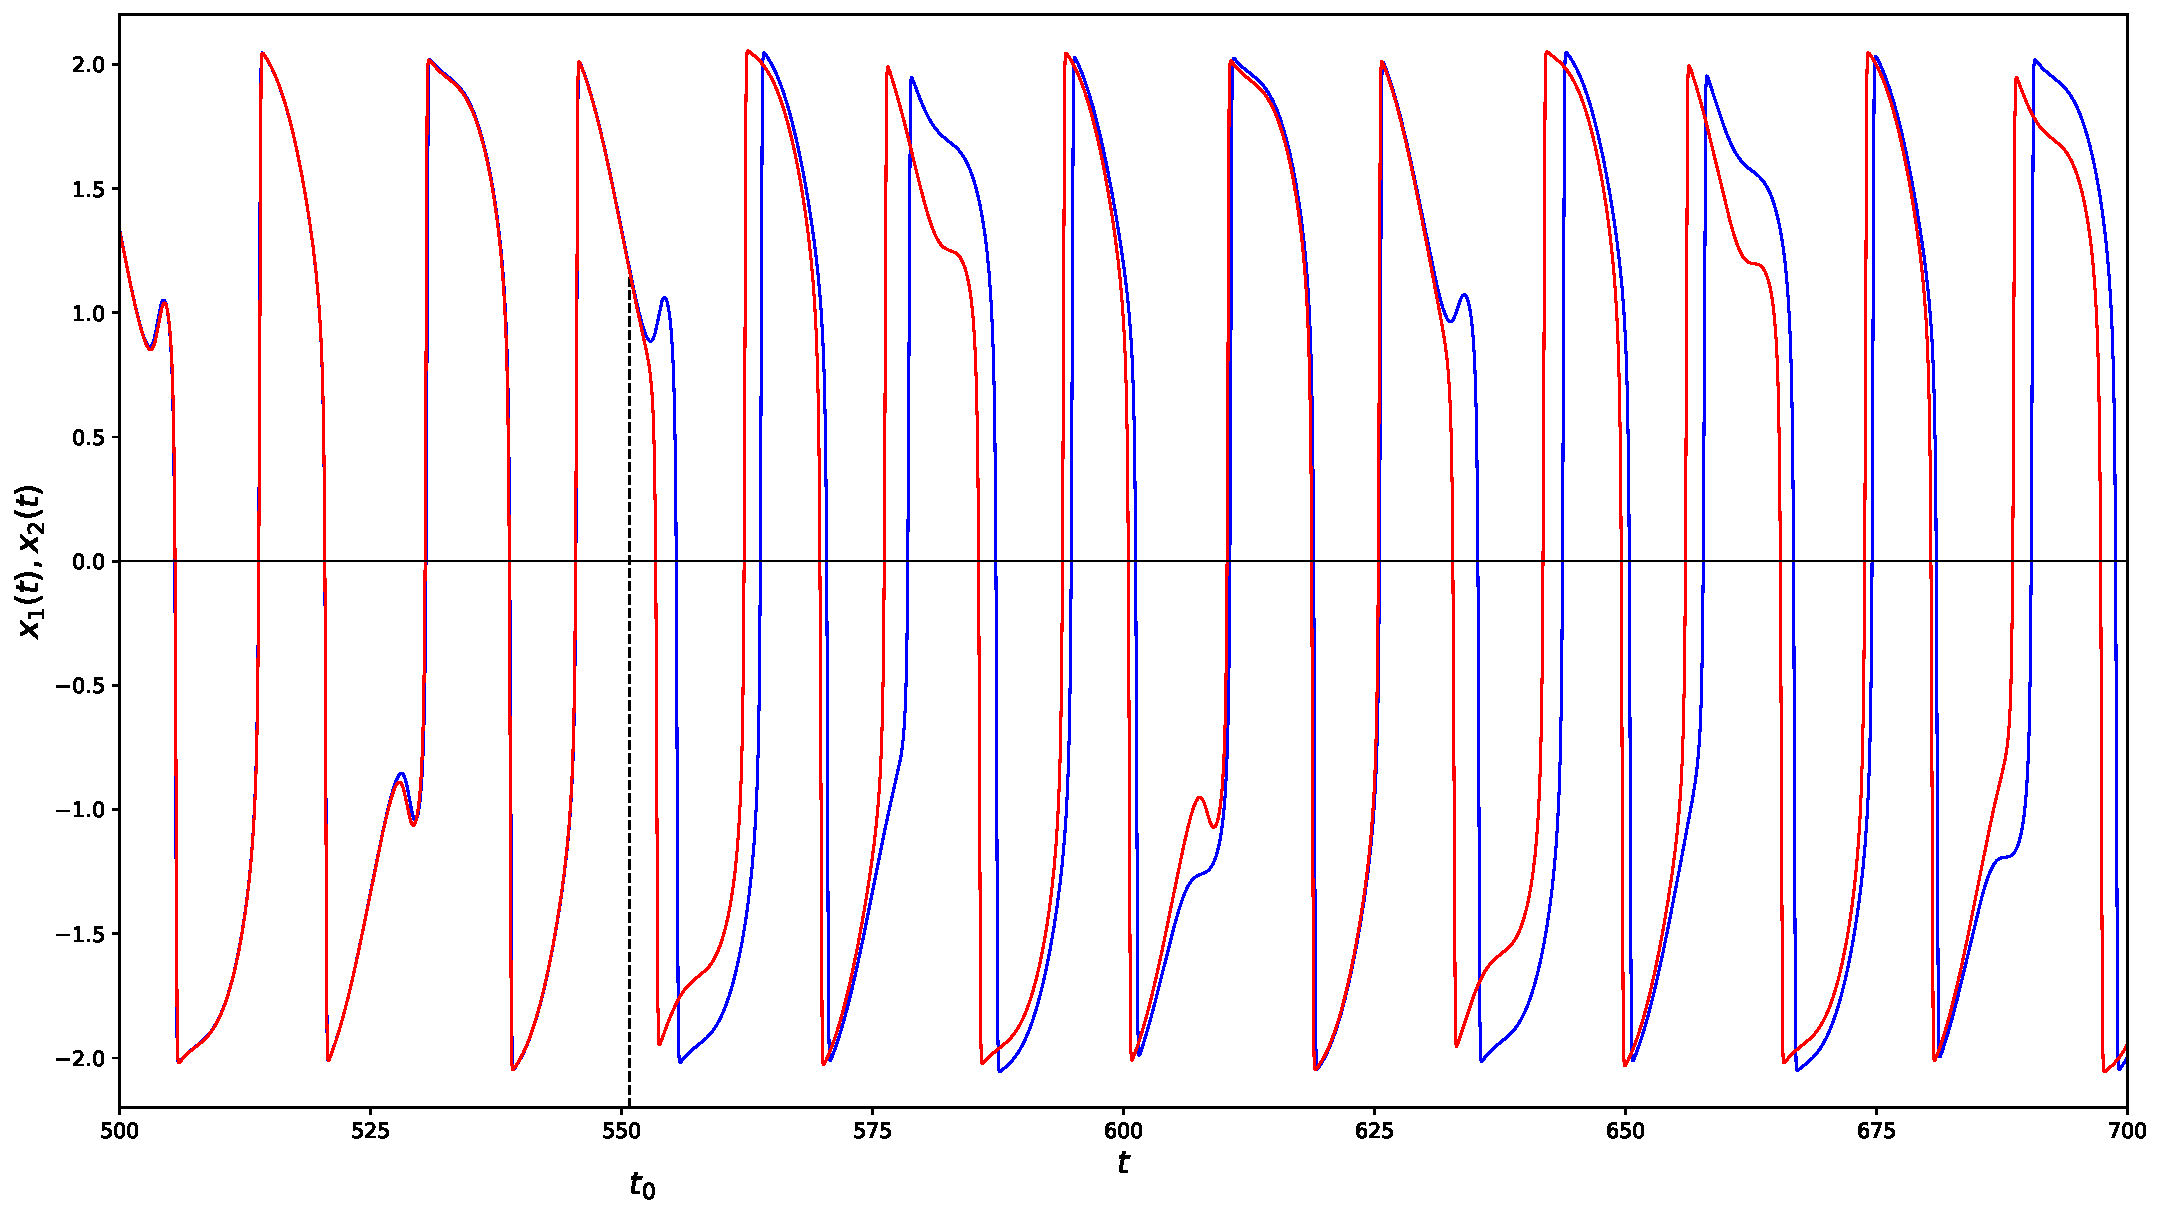
\includegraphics[width=\textwidth]{papers/vanderpol/figures/RK_schritt_delta_2e-3_2.pdf}
\caption{Verlauf der beiden mit der Runge-Kutta-Methode vierter Ordnung berechneten Lösungen $x_1$ und $x_2$ im Zeitbereich und Angabe des Divergenzpunktes $t_0$. Integrationsschritte: $h_1 = 0.007, \quad h_2 = 0.009$\label{vanderpol:figures:RK_schritt_2e-3}}
\end{figure}

\begin{figure}
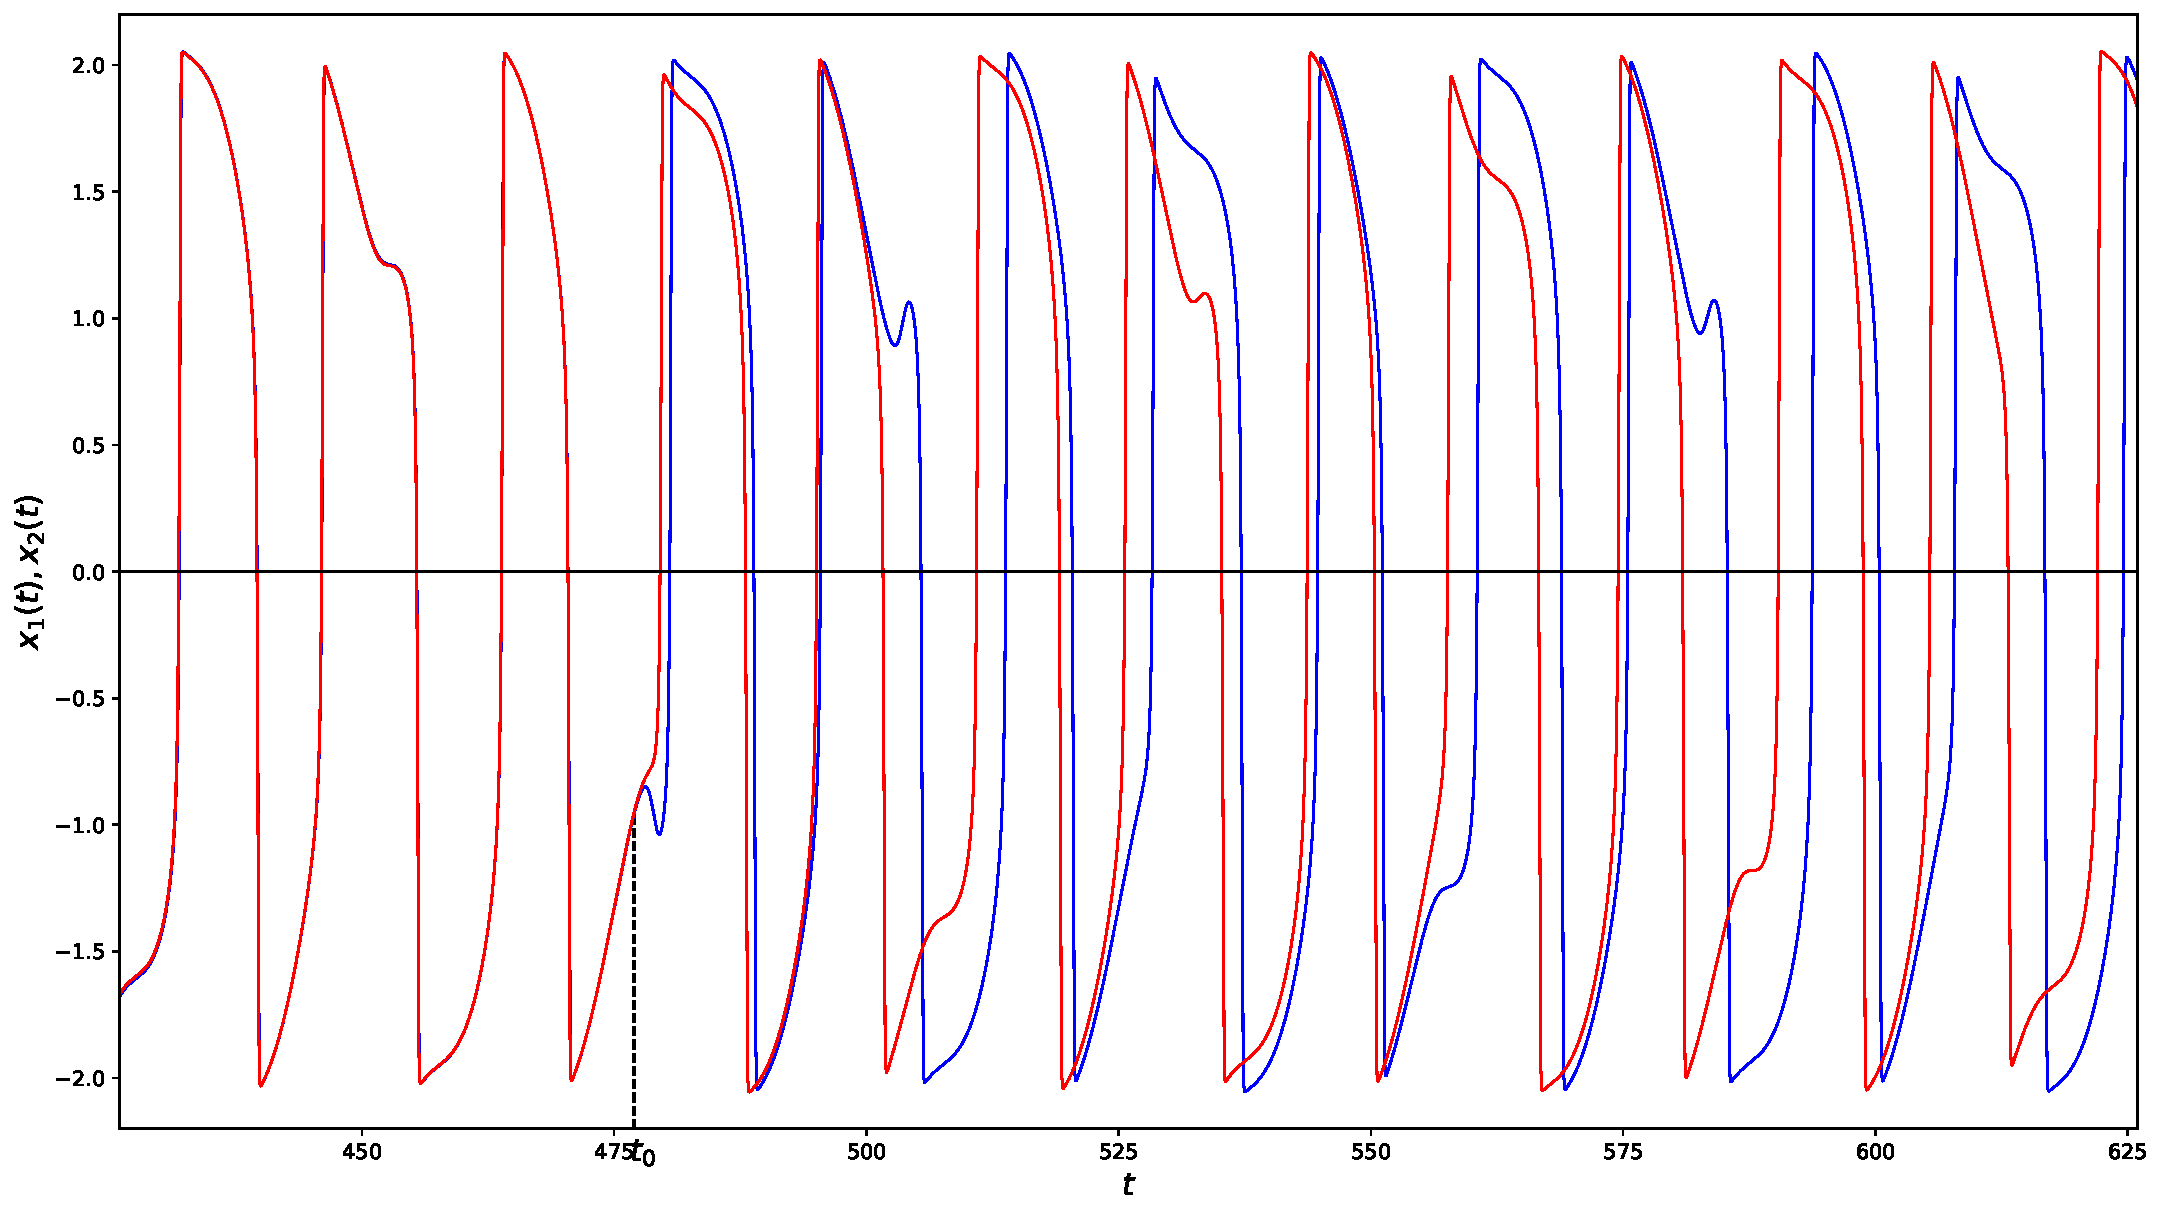
\includegraphics[width=\textwidth]{papers/vanderpol/figures/RK_schritt_delta_2e-3.pdf}
\caption{Verlauf der beiden mit der Runge-Kutta-Methode vierter Ordnung berechneten Lösungen $x_1$ und $x_2$ im Zeitbereich und Angabe des Divergenzpunktes $t_0$. Integrationsschritte: $h_1 = 0.005, \quad h_2 = 0.007$\label{vanderpol:figures:RK_schritt_2e-3_2}}
\end{figure}

